\normalfalse \difficiletrue \tdifficilefalse
\correctiontrue

%\UPSTIidClasse{11} % 11 sup, 12 spé
%\newcommand{\UPSTIidClasse}{12}

\exer{Mouvement RR 3D  $\star$ \label{B2:13:08}}
\setcounter{numques}{0}
\UPSTIcompetence[2]{B2-13}
\index{Compétence B2-13}
\index{Mécanisme à 2 rotations 3D}
\ifcorrection
\else
\textbf{Pas de corrigé pour cet exercice.}
\fi

\ifprof
\else
Soit le mécanisme suivant. On a $\vect{AB}=H\vect{j_1}+R\vect{i_1}$ et $\vect{BC}=L\vect{i_2}$. On a $H=\SI{20}{mm}$, $r=\SI{5}{mm}$, $L=\SI{10}{mm}$. 
\begin{center}
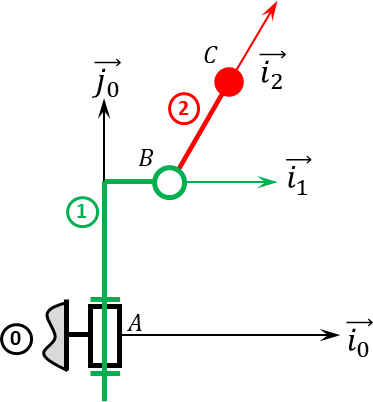
\includegraphics[width=\linewidth]{08_RR3D_01}
\end{center}
\fi

\question{Déterminer $\vectv{C}{2}{0}$ par dérivation vectorielle.} 
\ifprof
$\vectv{C}{2}{0}$ 
$=\deriv{\vect{AC}}{\rep{0}}$
$=\deriv{H\vect{j_1}+R\vect{i_1}+L\vect{i_2}}{\rep{0}}$.

Calculons : 
\begin{itemize}
\item $\deriv{\vj{0}}{\rep{0}}$ $=\vect{0}$;
\item $\deriv{\vi{1}}{\rep{0}}$ $=\vecto{1}{0} \wedge \vi{1}$ $=\dot{\theta}\vj{1} \wedge \vi{1}$ $=-\dot{\theta}\vk{1}$;
\item $\deriv{\vi{2}}{\rep{0}}$ $=\vecto{2}{0} \wedge \vi{2}$ 
$=\left(\dot{\theta}\vj{1} + \dot{\varphi}\vk{2}\right)\wedge \vi{2}$
$=\dot{\theta}\vj{1}\wedge \vi{2} + \dot{\varphi}\vk{2}\wedge \vi{2}$
$=-\dot{\theta}\cos\varphi\vk{1} + \dot{\varphi}\vj{2}$.
\end{itemize}

On a donc 
$\vectv{C}{2}{0}$ 
$= -R\dot{\theta}\vk{1}+L\left(-\dot{\theta}\cos\varphi\vk{1} + \dot{\varphi}\vj{2}\right)$.


\else
\fi

\question{Déterminer $\vectv{C}{2}{0}$ par composition du vecteur vitesse.} 
\ifprof
$\vectv{C}{2}{0}=\vectv{C}{2}{1}+\vectv{C}{1}{0}$.

\begin{itemize}
\item Pour calculer $\vectv{C}{2}{1}$, passons par $B$ car $\vectv{B}{2}{1}=\vect{0}$ :
$\babarv{C}{B}{2}{1}$
$ = \vect{CB}\wedge\vecto{2}{1}$
$ = -L\vi{2}\wedge\dot{\varphi}\vk{2}$
$ = L\dot{\varphi}\vj{2}$.
\item Pour calculer $\vectv{C}{1}{0}$, passons par $A$ car $\vectv{A}{1}{0}=\vect{0}$ :
$\babarv{C}{A}{1}{0}$
$ = \vect{CA}\wedge\vecto{1}{0}$
$ = -\left( H\vect{j_1}+R\vect{i_1}+L\vect{i_2}\right)\wedge\thetap\vj{1}$
$ = -\thetap\left( R\vect{i_1}\wedge\vj{1}+L\vect{i_2}\wedge\vj{1}\right)$
$ = -\thetap\left( R\vk{1}+L\cos\varphi\vk{1}\right)$.
\end{itemize}

Au final, $\vectv{C}{2}{0}= L\dot{\varphi}\vj{2}-\thetap\left( R\vk{1}+L\cos\varphi\vk{1}\right)$.
\else
\fi

\question{Donner le torseur cinématique $\torseurcin{V}{2}{0}$ au point $C$.}
\ifprof~\\
$\torseurcin{V}{2}{0}=\torseurl{\dot{\varphi}\vk{2}+\thetap\vj{0}}{ L\dot{\varphi}\vj{2}-\thetap\left( R\vk{1}+L\cos\varphi\vk{1}\right)}{C}$.

\else
\fi

\question{Déterminer $\vectg{C}{2}{0}$.}
\ifprof ~\\
$\vectg{C}{2}{0} =\deriv{\vectv{C}{2}{0}}{\rep{0}}$

$ =\deriv{ L\dot{\varphi}\vj{2}-\thetap\left( R\vk{1}+L\cos\varphi\vk{1}\right)}{\rep{0}} $.

Calculons :
\begin{itemize}
\item $\deriv{\vj{2}}{\rep{0}}=\vecto{2}{0}\wedge\vj{2}$ 
$=\left(\thetap\vj{1}+\thetap\vk{1} \right)\wedge\vj{2}$ 
$=\thetap\vj{1}\wedge\vj{2}+\thetap\vk{1} \wedge\vj{2}$
$=\thetap\sin\varphi\vk{1}-\thetap\vi{2} $.
\item $\deriv{\vk{1}}{\rep{0}} = \thetap\vi{1}$.
\end{itemize}

$\vectg{C}{2}{0} $
$ =
L\ddot{\varphi}\vj{2}+L\dot{\varphi}\left(\thetap\sin\varphi\vk{1}-\thetap\vi{2}\right)
-\thetapp\left( R\vk{1} +L\cos\varphi\vk{1}\right)
-\thetap\left( R \thetap\vi{1} +L\cos\varphi \thetap\vi{1}
-L\varphip\sin\varphi\vk{1}\right)
$.
\else
\fi


\ifprof
\else
\footnotesize
\begin{center}
\begin{tabular}{|p{.9\linewidth}|}
\hline
Indications :
\begin{enumerate}
\item $\vectv{C}{2}{0}= -R\dot{\theta}\vk{1}+L\left(-\dot{\theta}\cos\varphi\vk{1} + \dot{\varphi}\vj{2}\right)$.
\item $\vectv{C}{2}{0}= L\dot{\varphi}\vj{2}-\thetap\left( R\vk{1}+L\cos\varphi\vk{1}\right)$.
\item $\torseurcin{V}{2}{0}=\torseurl{\dot{\varphi}\vk{2}+\thetap\vj{0}}{ L\dot{\varphi}\vj{2}-\thetap\left( R\vk{1}+L\cos\varphi\vk{1}\right)}{C}$.
\item $\vectg{C}{2}{0} =
L\ddot{\varphi}\vj{2}+L\dot{\varphi}\left(\thetap\sin\varphi\vk{1}-\thetap\vi{2}\right)
-\thetapp\left( R\vk{1} +L\cos\varphi\vk{1}\right)
-\thetap\left( R \thetap\vi{1} +L\cos\varphi \thetap\vi{1}
-L\varphip\sin\varphi\vk{1}\right)$.
\end{enumerate} \\ \hline
\end{tabular}
\end{center}
\normalsize
\begin{flushright}
\footnotesize{Corrigé  voir \ref{B2:13:08}.}
\end{flushright}%
\fi